\documentclass[final,12pt]{elsarticle}
\usepackage{latexsym}

\usepackage{amsmath,amssymb} 
\usepackage[figuresright]{rotating}
\usepackage{epsfig}
\usepackage{graphicx}
\usepackage{longtable}
\usepackage{enumerate}
\usepackage{wrapfig}
\usepackage{subfigure}
\usepackage{array}
\usepackage{multirow,bigstrut,bigdelim}
\usepackage{tabularx}
\usepackage[T1]{fontenc}
\usepackage{color}
\usepackage{adjustbox}
\usepackage{caption}

\newcommand{\f}{\footnote}
\newcommand{\comm}[1]{}



\renewcommand{\figurename}{Fig.}

\newcommand{\be}{\begin{equation}}
\newcommand{\ee}{\end{equation}}
\newcommand{\bea}{\begin{eqnarray}}
\newcommand{\eea}{\end{eqnarray}}

\begin{document}


\begin{frontmatter}

\title{Calculation of Electrical Resistivity of Liquid Alkali Metals Na and Cs}


%\maketitle

\begin{abstract}
Electrical resistivity, $\rho$ of liquid alkali metals Na and Cs are calculated by using Bretonnet-Silbert (BS) pseudo-potential for inter-ionic interaction and LWCA (Linearised Weeks-Chandler-Anderson) perturbation theory for liquid structure. Ichimaru \& Utsumi (IU) and Vashishta \& Singwi (VS) screening functions are used to observe the effect of dielectric function in the potential. Applying form factor $V(q)$ (Fourier transform of potential $V(r)$) and partial structure factor $S(q)$,we compare our resistivity data of Cs and Na with available experimental and other theoretical data which shows good qualitative consistency with experimental data. We observe that VS screening function with LWCA theory provides the same results as IU for Cs and Na.

\end{abstract}

\begin{keyword}
Electrical resistivity \sep Alkali metals \sep Transport properties \sep Pair correlation function \sep Static structure factor \sep Hard sphere diameter
\end{keyword}

\end{frontmatter}

\section{Introduction}

Because of their thermal, electrical, mechanical and optical qualities, metals have a wide range of uses in science and technology.Scientists, metallurgists and technologists have been drawn to liquid metals at or near room temperature because of their softness and fluidity in reaction to stress.Stretchability, deformability, injectability and shape-reconfigurability are all possibilities for metals.These physical characteristics help soft sensors, electrical or optical components in microfluidic channels, and conductors in flexible or reconfigurable electronics.Metals that melt at high temperatures are utilized in nuclear reactors like NaK~\cite{Dickey2014} to convert heat and to make metal parts.Alkali metals, like other metals, are highly conductive and corrosion resistant, both of which are crucial characteristics in technology.


Upon considering the wide application of liquid metals and to understand their stucture, Scientists studied structural~\cite{Bhuiyan1996}, thermodynamic~\cite{Bhuiyan2000,Zahid1999}, electron transport properties~\cite{Sharmin2002} and  atomic transport properties~\cite{Bhuiyan2003,Gosh2013,Bhuiyan2008} of liquid simple metals. 

The static structural factor~\cite{Leavens1981,Nardi1996}is usually a limiting factor in calculating electron transport parameters. Various methodologies~\cite{Hansen1976} have been proposed i.e. Perturbation theories~\cite{Week1971,Ishihara1968,Barkar1967}, integral equation theories~\cite{Bhuiyan1993} and computer simulation method~\cite{McGreevey1991} have been developed to characterize the liquid structure.As a result of the above success, we use the HS theory within the Percus-Yevick approximation 'HSPY' as the reference system in this work instead of experimenting with alternative reference systems. There are many theoretical and experimental evidences~\cite{Waseda,Shimoji39} that the HS model can describe the structure of simple liquid metals reasonably well. In particular, a recent work~\cite{Khaleque2002} showed nicely that the mixture of two HS liquids with different effective diameters described the structure of liquid.
The static structural factor is usually a limiting factor in calculating electron transport parameters~\cite{Leavens1981,Nardi1996}. Various methodologies~\cite{Hansen1976} have been proposed i.e. Perturbation theories~\cite{Week1971,Ishihara1968,Barkar1967}, integral equation theories~\cite{Bhuiyan1993} and computer simulation method~\cite{McGreevey1991} have been developed to characterize the liquid structure.  The HS model can reasonably represent the structure of simple liquid metals, according to several theoretical and experimental evidences~\cite{Waseda,Shimoji39}. As a result of the above success, we use the HS theory within the Percus-Yevick approximation 'HSPY' as the reference system in this work instead of experimenting with alternative reference systems~\cite{Ross40,Hafner41}. The effective HS diameter, or 'HSD,' is necessary to characterize the HSPY liquid system and we determined it using the linearized Week-Chandler-Andersen 'LWCA' theory. The WCA theory~\cite{Mayer1980}, which was initially applied to elemental simple metallic systems by Kumaravadivel and Evans~\cite{Kumar23} to the elemental simple metallic systems,which is the foundation of the LWCA theory.This theory have been successfully applied at~\cite{Gosh2007,Bhuiyan2003} to the study of various material properties.
%transport

The key to study electron transport theory in metals is the electron-ion pair potential~\cite{Rossiter1991}.As a result, in order to investigate the electronic transport features of the relevant systems, an appropriate potential is required to adequately explain the interaction between atoms.
Physicists frequently use the pseudo-potential method.
It has been effectively used to investigate various properties of liquid metals~\cite{Fiolhais1996,Fiolhais1995,Sinclair1984,Daw1984,Walter1966,Hohenberg1964,Kohn1965,Mermin1965}. In this context, the Bretonnet and Silbert(BS) model potential ~\cite{Bret1992} is an excellent candidate in this regard.The capacity of the BS model potential to accommodate both sp and d-band contributions individually inside the pseudo-potential formalism makes it unique. For liquid metals, the BS model has already proven to be useful in explaining liquid structure~\cite{Zahid1999,Khaleque2002}, electrical resistivity~\cite{Sharmin2002} and atomic transport properties~\cite{Bhuiyan2003}. The BS pseudo-potential has been effectively used in the investigation of atomic transport properties for alkali metals. ~\cite{MSU2018}. For precise quantitative analysis, pseudo-potential has to take into account of the exchange and correlation effect. Ichimaru-Utsumi (IU)~\cite{ichimaru} and Vashishta-Shingwi (VS)~\cite{Vashishta1972} are two sophisticated local field correction functions that meet the compressibility sum rule's self consistency.

Ziman's theory ~\cite{ziman1961} is a well-known formula for calculating electrical resistivity in the context of the nearly free electron (NFE) model.The first-order time-dependent perturbation theory~\cite{Baym1964} is the starting point for Ziman's formula.
This theory is based on the Long Mean Free Path (MFP) approximation.
As a result, a weak scattering picture emerges and Born approximation is valid.
Alkali metals have a mean free path that is hundreds of times their respective inter-atomic distance.
 

Alkali metals are highly reactive~\cite{feitsma1975}. Experimentation is therefore difficult.
It takes a long time to run a computer simulation.
As a result, theoretical technique is the most effective. 

To compute the electrical resistivity of all alkali metals, a comprehensive/holistic approach is required.
The precise combination of potential and liquid structure for alkali metals is what we meant by the term 'wholesome/holistic.'
We try to do so in this study by employing the BS pseudo-potential and the LWCA perturbative approach for liquid structure.
We also employed two other local field correcion functions, IU and VS, to improve the results.Sharmin et. al.~\cite{Sharmin2002} recently employed the BS pseudo-potential with the Ziman formula to study liquid less simple metals.
Their findings are consistent with the experiment.
We use the Bretonnet-Silbert pseudo-potential for electron-ion interaction and the LWCA perturebation theory for liquid structure to determine electrical resistivity of alkali metals. 

We measured electrical resistivity quantitatively for alkali metals like Na and Cs in this article. We used Ziman's method~\cite{ziman1961}to determine electrical resistivity for Cs and Na.

\section{Theories}
In the following we present briefly the electronic resistivity of K and Li
\label{theory}
\subsection{Bretonnet and Silbert model potential}
For simple system of alkali metals, Bretonnet and Silbert (BS) have proposed a pseudopotential model that considers both contributions from the $s$-$p$ and $d$- bands as
\begin{equation}
v(r) = \left\{ \begin{array}{ll}
\sum_{m=1}^{2}B_{m}\exp(-\frac{r}{ma}) & \mbox{for $r < R_{c}$} \\
-\frac{Z_{s}e^{2}}{r} & \mbox {for $r > R_{c}$}\end{array}\right.
\end{equation}.
where, $a$, $Z_{s}$ and $R_{c}$ represent the softness parameter, effective $s$-electron occupancy number and core radius, respectively. The unscreened form factor is given by
\begin{equation}
V_{0}(q)=4\pi na^{3}\Bigg[\frac{B_{1}J_{1}}{(1+a^{2}q^{2})^{2}}+\frac{8B_{2}J_{2}}{(1+4a^{2}q^{2})^{2}}\Bigg]-\frac{4\pi n Z_{s}e^{2}\cos(qR_{c})}{q^{2}},
\end{equation}
 the expressions for $B_{m}$ and $J_{m}$ are given
in~\cite{Bret1992}. Therefore the effective interionic interaction is given by
\begin{equation}
v(r)=\frac{Z_{s}^{2}e^2}{r}\Bigg(1-\frac{2}{\pi}\int F_{N}(q)\frac{\sin(qr)}{q}dq\Bigg)
\end{equation}
where $F_{N}(q)$ denotes the normalized energy wave number characteristic.It has the following form,
\begin{equation}
F_{N}(q)=\Bigg(\frac{q^{2}}{4\pi n Z_{s}e^{2}}\Bigg)^{2}w_{0}^{2}(q)\Bigg[1-\frac{1}{\epsilon(q)}\Bigg][1-G(q)]^{-1}.
\end{equation}


 $\epsilon(q)$ denotes the dielectric screening function is and it is given by
 
 
\begin{equation}
\label{EP0}
\varepsilon(q)=1-\Bigg[\frac{\frac{4\pi e^{2}}{q^{2}}\chi(q)}{1+\frac{4\pi e^{2}}{q^{2}}G(q)\chi(q)}\Bigg],
\end{equation} 
where $\chi(q)$ denotes the Lindhard function.$G(q)$ is the local-field correction and it was developed by Ichimaru and Utsumi (IU)~\cite{Ichimaru1981}.
\subsection{LWCA Perturbation theory}
The WCA theory~\cite{Week1971} is the starting point for the LWCA thermodynamic perturbation method as proposed by Meyer et al.~\cite{Mayer1980}. The blip function in WCA theory~\cite{Week1971} is given as
\begin{equation}
\label{blip}
B(r)=Y_{\sigma}(r)[\exp(-\beta v(r))-\exp(-\beta V(r))]
\end{equation}
where $v(r)$ and $V(r)$ are the soft and the hard sphere potentials, respectively. $\beta$ denotes the inverse temperature times Boltzmann constant. In Eqn.~(\ref{blip}), $Y_{\sigma}(r)$ is the cavity function associated with HS distribution function and continuous at $r$ = $\sigma$. Within the linearised WCA approximation, thermodynamic condition that for an effective hard sphere diameter (HSD), $B(q = 0)$ vanishes leads to the transcendental equation
\section{Static structure factor}
The Ashcroft and Langreth (AL) partial structure factors S are calculated with their original work~\cite{LAshcroft1967} 
\begin{equation}
S(q)=1+n {(c^2)}^{1/2} \int[g(r)-1]\exp [i\bar q.\bar r]d^{3}r
\end{equation}
where $S(q)$ is the hard-sphere momentum-space solutions of the Percus-Yevick (PY) equation appropriate to our simple systems . 

 The value of the HSD are determined by using linearized Weeks-Chandler-Anderson (LWCA) perturbation theory. 
\
\section{Electrical resistivity of liquid metals}
The famous Ziman's formula for electrical resistivity of simple metals:
\be
\label{zn}
\rho=\frac{3\pi m^2}{4Ze^2\hbar^3 n k^6_{\rm F}} \int_{0}^{\infty} q^3S(q){\lvert{V(q)}\rvert}^{2} dq
\ee
Where $S(q)$, $V(q)$,$q$,$Z$,$n$,$e$,$m$ represent the static structure factor, screened form factor in q-space, the momentum transfer, effective s-electron occupancy number, conduction electron density, electron charge and effective mass, respectively. At high temperature, the effective mass approaches to the free electron mass~\cite{Baym1964}. So, in this work we approximated the effective mass is equal to the free electron mass. We have also truncated the integrand at $q$ = 2$k_{\rm F}$ resulting a perfect sharp fermisurface. It is considered that the wave vectors q of electrons lying on the fermi surface are responsible for the scattering. The conduction electron density can be represented as a function of wave vector $k_F$ , $n$= 3$\pi^2$/$k_{\rm F}^3$ .

\section{Results and Discussion}
\label{res}
In this section, we first gave a theoretical calculation of alkali metal resistivity, followed by a discussion of the results.
As previously stated, the form factor,$V(q)$ and structure factor $S(q)$are the most important components of this computation.
The BS pseudo-potential is intimately related to both the form factor and the static structure factor.
Three parameters , $R_c$, $a$ and $Z$ are the most important components of this computation.
The BS pseudo-potential is intimately related to both the form factor and the static structure factor.
Three parameters must be fixed for BS pseudo-potential, according to the following:
Fitting to the the values of physical qualities $R_c$  of the system of interest is the most common method of determining them.
 Bhuiyan et. al.~\cite{Bhuiyan1993}'s  procedure is used to determine the results.The values of $R_c$ and $a$ Waseda et. al.~\cite{Waseda}'s experimental value was fitted to the structure factor for our concerned systems as shown in Fig.\ref{pfig1}. The Z values represent $sp$-$d$ hybridization effect. Z values for alkali metals are treated as Z = 1.0, assuming no $sp$-$d$ hybridization. The formula from ref~\cite{Smithells} is used to calculate number densities. Table~\ref{t1} lists the values of the input parameters~\ref{t1}. 

We construct effective partial pair potential $V(r)$ from the BS model potential to evaluate partial inter-ionic interaction.
The choice of electron gas dielectric function has a big impact on $V(r)$.  As a result, we've included two separate local field correction functions:  Ichimaru and Utsumi (IU)~\cite{ichimaru} and Vashishta and Singwi (VS)~\cite{Vashishta1972}. In (c) and (d) of Fig.~\ref{pfig1} the partial pair potentials $V(r)$ and screening form factor $V(q)$ derived using IU for Na are displayed.Figure~\ref{pfig1} illustrates this point Hence the depth of the potential well is lowest for $V 11(r)$ and highest for $V 22(r)$; $V 12(r)$ lies in the middle.
This is due to the complex balance between the repulsive and attractive interactions in metals, which determines the depth of the potential well and the location of major minima.
These interactions occur in the pseudo-potential formalism due to direct interaction between various ion-cores and indirect interaction via conduction electrons.In this case, the dielectric function is quite critical.  

When VS is used instead of IU, the depth of the potential well is increased, and the position of the primary minima shifts somewhat toward increasing $r$, but otherwise all alloys in our concerned systems follow the same trends as IU.  

The hard sphere diameter (HSD) values are derived using LWCA perturbative theory in order to calculate the static structure factor, $S(q)$.
As a representative example, $S(q)$ for concentration of 0.1 of Na$ x$Cs$ 1-x$ alloys are illustrated in Fig.~\ref{pfig2} (a) and Fig.~\ref{pfig5} (a) .For $x$ = 0.1, $S 22(q)$ has the biggest peak and $S 11(q)$ has the smallest, as seen in Fig.~\ref{pfig3}(a). It means that the chance of discovering ions near other ions is determined by both component concentration and HSD.
  
We estimated the resistivity of Cs and Na using the screened form factor $V(q)$ and the structure factor $S(q)$, as indicated in Fig.~\ref{pfig3} and Fig.~\ref{pfig6}.

To calculate the resistivity of Na and Cs we will use the method used in calculating the resistivity of Na$_x$Cs$_{1-x}$ alloy.

IN Fig.~\ref{pfig3} and Fig.~\ref{pfig6} and table ~\ref{t2} The resistivity of Na and Cs studied by us was compared to experimental and other theoretical values. For both IU and VS, the obtained results are superior to any other theoretical results.The results of VS are comparable to those of IU. 

We utilized 373K as the input temperature for Na a Cs to include all of the components in the liquid state.
As a result, we might conclude that the theories in use are valid at the given temperature.
We also compared the estimated resistivity to the experimental resistivity ~\ref{t2} for Na and Cs. As a result, LWCA is unable to provide accurate statistics for temperatures that are well below melting for liquid metals.
Otherwise, our findings are in line with those of the experiment. 

For the systems in concern, the static structure factor for Na is excellent, but Cs's result is deviated in this area.
This may also have an impact on our final result.
Second, it's worth noting that the static structural factor data we compared to the experimental data from Geertsma et. al.~\cite{{GGG2001}.  The potential parameters at the above stated temperature are calculated at slightly different temperatures than ours, such as 373K for Na and Cs, which could account for the variance. 

In every case, Both the results of  IU and VS are close to the experiment.But  Vs can predict better result by slight difference than IU in this study. 

\newpage
\begin{table}[htp]
\vskip -0.0cm
\begin{center}
%\tabcolsep=0.05cm
\caption{Values of the input parameters}
\label{t1}
\vspace{7mm}
\begin{tabular}{cccccc}\hline
Metal & $T_{0}$(K)  & $n$(\AA$^{-3}$)   &  $R_{c}$ ($a.u.$)  &   $a$ ($a.u.$) & $Z_{s}$  \\ \cline{1-6}
Na   &  373        & 0.0242            &   1.71   & 0.362      &  1.0       \\
Cs   &  373       & 0.00813            &   3.28    & 0.788     &  1.0        \\\hline
\end{tabular}
\end{center}
\end{table}


\begin{table}[htp]
	\vskip -0.0cm
	\begin{center}
		%\tabcolsep=0.05cm
		\caption{Resistivity values obtained from this  study}
		\label{t2}
		\vspace{7mm}
		\begin{tabular}{cccccc}\hline
			Metal & $T_{0}$(K)  &     & &  $\rho$ (micro ohm-cm)  \\
			\\
			\cline{1-6}
			\\
			 \multirow{} &  &   IU \doublespace &VS&exp&theo \\ 
			 \cline{1-6}
			 \\
			Cs   & 373      &   9.913   & 9.913      &      36.0       \\
			Na    & 373      &  3.909	& 3.909	      &    9.6        \\

                   \\
	        \\\hline
		\end{tabular}
	\end{center}
\end{table}
\begin{figure}[htp]
\begin{center}
\begin{tabular}{llll}
\vspace{-2.0cm}
\\(a) & (b) \\
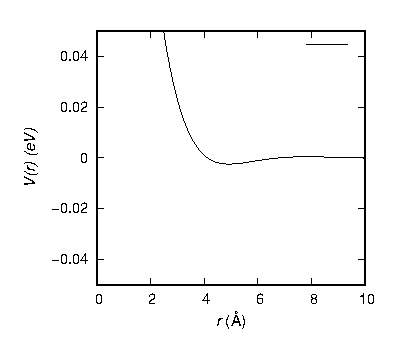
\includegraphics[width=7.4cm]{iCsBRET.eps}&
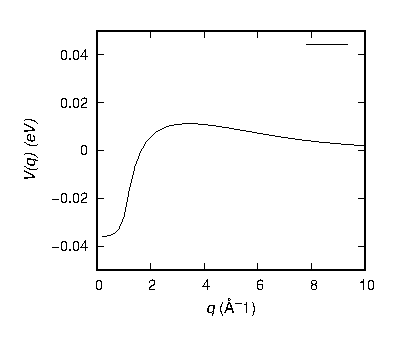
\includegraphics[width=7.4cm]{iCsFFACT.eps}\\&\\&\\
\vspace{-2.0cm}
\\(c) & (d) \\
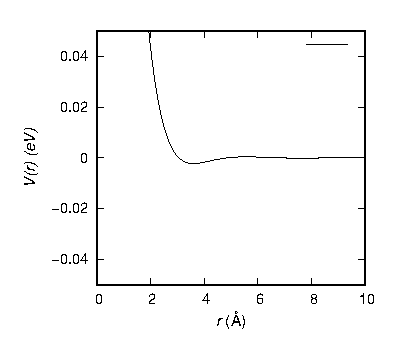
\includegraphics[width=7.4cm]{iNaBRET.eps}&
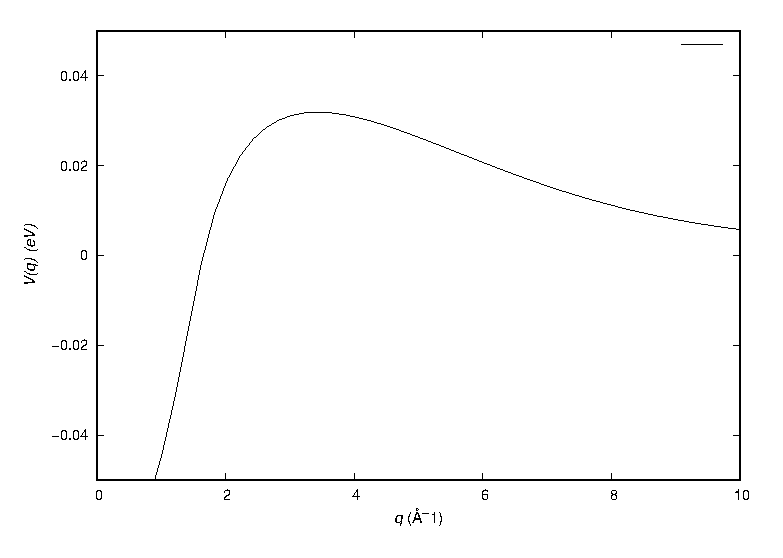
\includegraphics[width=7.4cm]{iNaFFACT.eps}\\&\\&\\

\end{tabular}
\caption{Fig(a) and (c) are the $r$ Vs $V(r)$ graph and (b) and (d) are the $q$ Vs $V(q)$ graph of Cs and Na .}
\label{pfig1}
\end{center}
\end{figure}

\begin{figure}[htp]
\begin{center}
\begin{tabular} {lll}
\vspace{2.0cm}
\\(a)& (b) \\
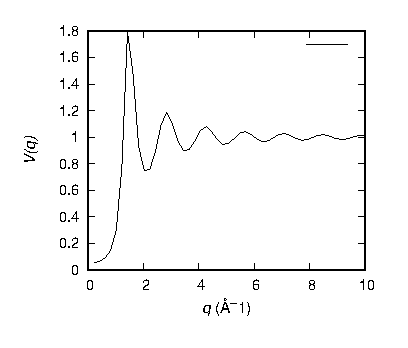
\includegraphics[width=7.4cm]{iCsS(q).eps}&
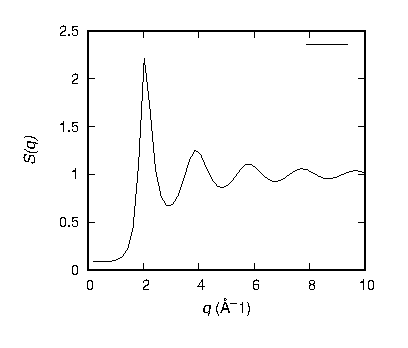
\includegraphics[width=7.4cm]{iNaS(q).eps}\\&\\&\\
\end{tabular}
\caption{Fig (a) and (b) are $ q $ Vs $V(q)$ graph of Cs and Na respectively.}
\label{pfig2}
\end{center}
\end{figure}

\begin{figure}[htp]
\begin{center}
\begin{tabular}
\vspace{-2.0cm}
\\(a)\\ 
\includegraphics[width=7.4cm,angle=-90]{irCs.eps}&
\\(b)\\
\includegraphics[width=7.4cm,angle=-90]{irNa.eps}\\&\\&\\
\vspace{-1.0cm}

\end{tabular}
\caption{This is the resistivity $\rho$ of Cs and Na in IU method}
\label{pfig3}
\end{center}
\end{figure}

\begin{adjustbox}{center,caption={This is the resistivity $\rho$ of Cs and Na in IU method},label={pfig3},vspace=\bigskipamount}
	\includegraphics[width=0.6\textwidth,angle=-90]{irCs.eps}
	\caption[short]{a}
	\includegraphics[width=0.6\textwidth,angle=-90]{irNa.eps}
	\caption{figure}{b}
\end{adjustbox}

\begin{adjustbox}{center,label={somelabel},vspace=\bigskipamount}
	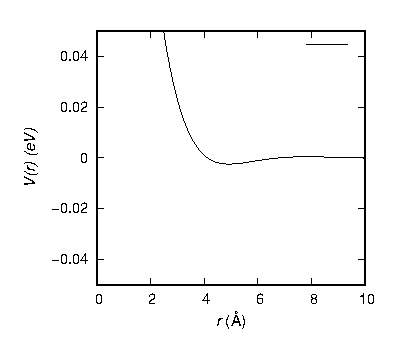
\includegraphics[width=0.6\textwidth]{vCsBRET.eps}
	\caption[short]{a}
	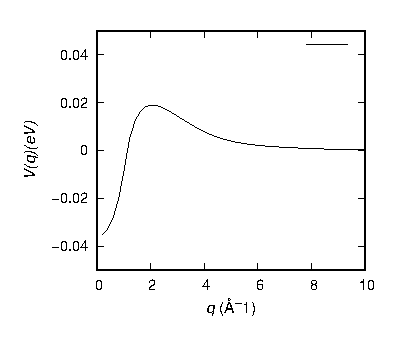
\includegraphics[width=0.6\textwidth]{vCsFFACT.eps}
	\caption{figure}{b}
\end{adjustbox}

\begin{adjustbox}{center,caption={Fig(a) and (c) are the $r$ Vs $V(r)$ graph and (b) and (d) are the $q$ Vs $V(q)$ graph  of Cs and Na.},label={somelabel},nofloat=figure,vspace=\bigskipamount}
	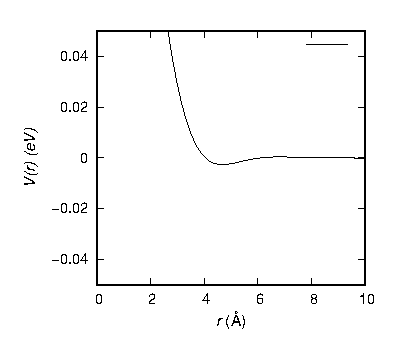
\includegraphics[width=0.6\textwidth]{vNaBRET.eps}
	\caption{figure}{c}
	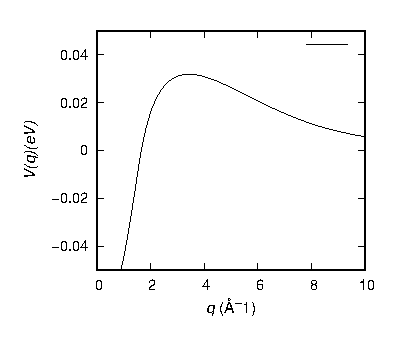
\includegraphics[width=0.6\textwidth]{vNaFFACT.eps}
	\caption{figure}{d}
\end{adjustbox}

\begin{adjustbox}{center,caption={Fig(a) and (c) are the $r$ Vs $V(r)$ graph and (b) and (d) are the $q$ Vs $V(q)$ graph  of Cs and Na.},label={somelabel},nofloat=figure,vspace=\bigskipamount}
	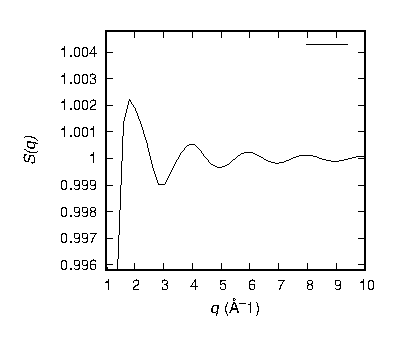
\includegraphics[width=0.6\textwidth]{vCsS(q).eps}
	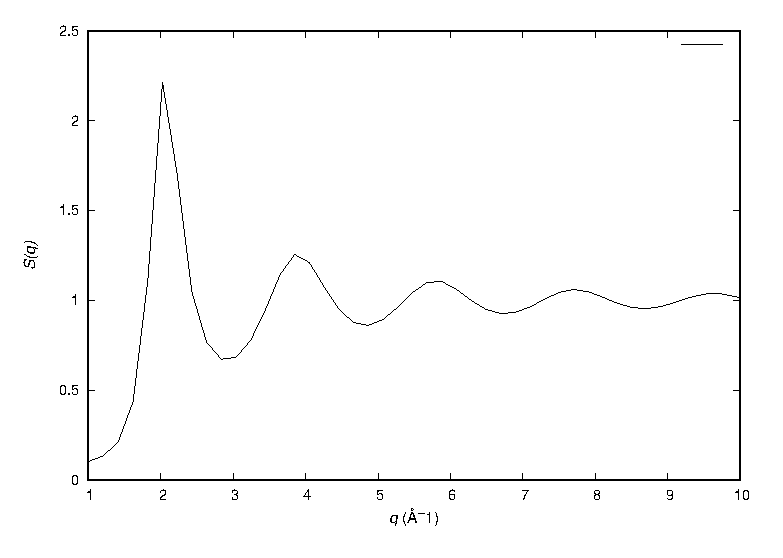
\includegraphics[width=0.6\textwidth]{vNaS(q).eps}
\end{adjustbox}

\begin{adjustbox}{center,caption={This is the resistivity ($\rho$) of Cs and Na in VS method},label={somelabel},nofloat=figure,vspace=\bigskipamount}
	\includegraphics[width=0.6\textwidth,angle=-90]{irCs.eps}
	\includegraphics[width=0.6\textwidth,angle=-90]{irNa.eps}
\end{adjustbox}

\begin{adjustbox}{center,caption={q Vs SS(q) graph for comparison of IU and VS method for Na},label={somelabel},nofloat=figure,vspace=\bigskipamount}
	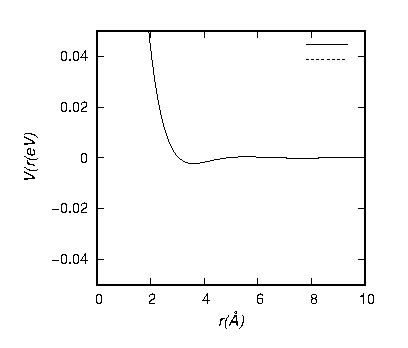
\includegraphics[width=\textwidth]{NacomBRET.eps}
\end{adjustbox}
\section{Conclusions}
\label{conclu}
In this paper, we have calculated the resistivity of metals using BS pseudo-potential and LWCA perturbative theory for liquid alkali metals which proves to be successful. Choice of local field corrections are important to get better resistivity results . In both VS and IUb gives same results. Regarding the case for small angle scattering, LWCA can not provide accurate static structure factor data that's why our results faces discrepancy. Among the metals Na and Cs resistivity results of Na is better than Cs inany other exiting theories for both local field correction functions. 
\newpage
\newpage

\begin{thebibliography}{thesis}
	
	\bibitem{Dickey2014}M. D. Dickey, Emerging Applications of Liquid Metals Featuring Surface Oxides, ACS Appl. Mater. Interfaces, 6 (2014), pp. 18369-18379; https://dx.doi.org/10.1021/am5043017. 
	\bibitem{Bhuiyan1996}G. M. Bhuiyan, M. Silbert, and M. J. Stott, Structure and thermodynamic properties of liquid transition metals: An embedded-atom-method approach, Phys. Rev. B 53, (1996), pp. 636; https://doi.org/10.1103/PhysRevB.53.636.
	\bibitem{Bhuiyan2000}G. M. Bhuiyan , A. Rahman , M. A. Khaleque , R. I. M. A. Rashid and S. M. Mujibur Rahman, Structural, Thermodynamic and Transport Troperties of Liquid Noble and Transition Metals, Phys. and Chem. of Liq., 38, 1 (2000),pp. 1-16,https://doi.org/10.1080/00319100008045292.
	\bibitem{Zahid1999}F.Zahid, G.M. Bhuiyan, S.Sultana, M.A. Khaleque, R.I.M.A. Rashid and S.M.M. Rahman, Investigations of the Static and Dynamic Properties of Liquid Less Simple Metals, Phys. Stat. Sol. B 215, 2 (1999), pp.987-998;https://doi.org/10.1002/(SICI)1521-3951(199910)215:2<987::AID-PSSB987>3.0.CO;2-E.
	\bibitem{Sharmin2002}S. Sharmin, G.M. Bhuiyana, M.A. Khaleque, R.I.M.A. Rashid, S.M.M. Rahman, Electronic transport properties of liquid less-simple metals, physica status solidi (b) 232 (2), (2002), pp. 243–253, https://doi.org/10.1002/1521-3951(200208)232:2<243::AID-PSSB243>3.0.CO;2-W.
	\bibitem{Bhuiyan2003}G.M. Bhuiyan, I. Ali and S.M.M. Rahman, Atomic transport properties of AgIn liquid binary alloys, Physica B: Condensed Matter, 334(1-2) (2003), pp. 147-159; https://doi.org/10.1016/s0921-4526(03)00040-1.
	\bibitem{Gosh2013}R.C. Gosh, M.R. Amin, G.M. Bhuiyan, Atomic transport for liquid noble and transition metals using scaling laws, Journal of Molecular Liquids, 188, (2013), pp. 148-154, https://doi.org/10.1016/j.molliq.2013.09.034.
	\bibitem{Bhuiyan2008}E.H. Bhuiyan,A.Z. Ziauddin Ahmed,G.M. Bhuiyan and M. Shahjahan, Atomic transport properties of Ag$_x$Sn$_{1-x}$ liquid binary alloys, Physica B: Condensed Matter, 403, 10-11 (2008), pp. 1695-1703, https://doi.org/10.1016/j.physb.2007.09.090.
	\bibitem{Leavens1981}C.R. Leavens, A.H. Mackdonald, R. Taylor, A. Ferraz and N.H.March, Finite Mean-Free-Paths and the Electrical Resistivity of Liquid Simple Metals, Phys. Chem. Liq. 11, 2 (1981) pp.115-128; https://doi.org/10.1080/00319108108079103.
	\bibitem{Nardi1996}E. Nardi, Plasma and liquid-metal resistivity calculations using the Ziman theory, Phys. Rev. E 54, 2 (1996)pp. 1899-1905;https://doi.org/10.1103/PhysRevE.54.1899
	\bibitem{Hansen1976}J.P. Hansen and J. R. McDonald, Theory of Simple Liquids, Academic Press, (1976).
	\bibitem{Week1971}J. D. Weeks, D. Chandler and H. C. Andersen,Role of Repulsive Forces in Determining the Equilibrium Structure of Simple Liquids, The Journal of Chemical Physics 54, (1971) 5237; https://doi.org/10.1063/1.1674820.
	\bibitem{Ishihara1968}A. Ishihara, The Gibbs-Bogoliubov inequality, J. Phys. , A1, (1968) 539.
	\bibitem{Barkar1967}J. A. Barker and D. Henderson, Perturbation Theory and Equation of State for Fluids. II. A Successful Theory of Liquids,The Journal of Chemical Physics 47, 4714 (1967); https://doi.org/10.1063/1.170168.
	\bibitem{Bhuiyan1993}G.M. Bhuiyan, J.L. Bretonnet and M. Silbert, Liquid structure of the 3d transition metals, J. Non-Cryst. Sol. 156-158 (1993), pp. 145-148; https://doi.org/10.1016/0022-3093(93)90149-R.
	\bibitem{McGreevey1991}R. L. McGreevy, Understanding liquid structures, Journal of Physics: Condensed Matter, 3(42), (1991) F9-F22; https://doi.org/10.1088/0953-8984/3/42/002.
	\bibitem{Waseda}Y. Waseda, The Structure of Non-crystalline Materials, McGraw Hill, Newyork, 55, 264 (1980).
	\bibitem{Shimoji39} M. Shimoji, Liquid Metals: An Introduction to the Physics and Chemistry of Metals in the Liquid States Academic, London, 1977, pp. 104-105.
	\bibitem{Khaleque2002}M. A. Khaleque, G. M. Bhuiyan, S. Sharmin, R. I. M. A. Rashid, and S. M. Mujibur Rahman, Calculation of partial structure factors of a less-simple binary alloy. The European Physical Journal B, 26(3) (2002), pp. 319-322; https://doi.org/10.1140/epjb/e20020095.
	\bibitem{Ross40}M. Ross, H. E. DeWitt, and W. B. Hubbard, Monte Carlo and perturbation-theory calculations for liquid metals, Phys. Rev. A 24 (1981), pp. 1016-1020; https://doi.org/10.1103/PhysRevA.24.1016.
	\bibitem{Hafner41}J. Hafner, A. Pasturel, and P. Hicter, Simple model for the structure and thermodynamics of liquid alloys with strong chemical interactions. II. Chemical order and packing constraints. Journal of Physics F: Metal Physics, 14(10) (1984), pp. 2279-2295; https://doi.org/10.1088/0305-4608/14/10/007.
	\bibitem{Mayer1980}A. Mayer, M. Silbert and W.H. Young, Chem. Phys. 49 (1980), pp. 147.
	\bibitem{Kumar23}R. Kumaravadivel and R. Evans, The entropies and structure factors of liquid simple metals, Journal of Physics C: Solid State Physics, 9(21) (1976), pp. 3877-3903; https//doi.org/10.1088/0022-3719/9/21/008.
	\bibitem{Gosh2007}R.C. Gosh, A.Z. Ziauddin Ahmed and G.M. Bhuiyan, Investigation of surface entropy for liquid less simple metals, The European Physical Journal B, 56(3) (2007), 177-181; https://doi.org/10.1140/epjb/e2007-00104-9.
	\bibitem{Rossiter1991}P.L. Rossiter, The Electrical Resistivity of Metals and Alloys, Cambridge University Press, Cambridge (1991).
	\bibitem{Fiolhais1996}C. Fiolhais, J.P. Perdew, S.Q. Armster, J.M. Maclaren and M. Brajczewska, Dominant density parameters and local pseudopotentials for simple metals, Physical Review B, 51(20) (1995), pp. 14001-14011; https://doi.org/10.1103/physrevb.51.14001.
	\bibitem{Fiolhais1995}C. Fiolhais, J.P. Perdew, S.Q. Armster, J.M. Maclaren and M. Brajczewska, Erratum: Dominant density parameters and local pseudopotentials for simple metals, Physical Review B, 53(19) (1995), pp. 13193-13193; https://doi.org/10.1103/physrevb.53.13193.
	\bibitem{Sinclair1984}M.W. Finnis and J.E. Sinclair, A simple empirical N-body potential for transition metals, Philosophical Magazine A, 50(1) (1984), pp. 45-55; https://doi.org/10.1080/01418618408244210.
	\bibitem{Daw1984}M.S. Dsw and M.I. Baskes, Embedded-atom method: Derivation and application to impurities, surfaces, and other defects in metals, Physical Review B, 29(12) (1984), pp. 6443-6453; https://doi.org/10.1103/physrevb.29.6443.
	\bibitem{Walter1966}Walter A. Harrison, Pseodopotentials in the theory of metals, W. A. Benjamin, Inc. (1966).
	\bibitem{Hohenberg1964}P. Hohenberg and W. Kohn, Inhomogeneous Electron Gas, Physical Review, 136(3B) (1964), pp. B864-B871; https://doi.org/10.1103/physrev.136.b864.
	\bibitem{Kohn1965}W. Kohn and L. J. Sham, Self-Consistent Equations Including Exchange and Correlation Effects, Physical Review, 140(4A) (1965), pp. A1133-A1138; https://doi.org/10.1103/physrev.140.a1133.
	\bibitem{Mermin1965}N. D. Mermin, Thermal Properties of the Inhomogeneous Electron Gas, Physical Review, 137(5A) (1965), pp. A1441-A1443; https://doi.org/10.1103/physrev.137.a1441.
	\bibitem{Bret1992}J.L. Bretonnet, G.M. Bhuiyan and M. Silbert, Gibbs-Bogoliubov variational scheme calculations for the liquid structure of 3d transition metals. Journal of Physics: Condensed Matter, 4(24) (1992), pp. 5359-5370; https://doi.org10.1088/0953-8984/4/24/005.
	\bibitem{MSU2018}Md Salah Uddin, R.C. Gosh, G.M. Bhuiyan, Investigation of surface tension, viscosity and diffusion coefficients for liquid simple metals, Journal of Non-Crystalline Solids, 499 (2018), pp. 426-433, https://doi.org/10.1016/j.jnoncrysol.2018.07.014.
	\bibitem{ichimaru}Ichimaru and K. Utsumi, Analytic expression for the dielectric screening function of strongly coupled electron liquids at metallic and lower densities, Physical Review B, 24(12) (1981), pp.  7385-7388; https://doi.org/10.1103/physrevb.24.7385.
	\bibitem{Vashishta1972}P. Vashishta and K.S. Singwi, Electron Correlations at Metallic Densities. V., Physical Review B, 6(3) (1972), pp. 875-887; https://doi.org/10.1103/physrevb.6.875.
	\bibitem{Mishra1990}A.K. Mishra, B.B. Sahay and K.K. Mukherjee, Structure and Electrical Resistivity of Alkali–Alkali and Lithium-Based Liquid Binary Alloys, Physica Status Solidi (b), 157(1) (1990), pp. 85-92; https://doi.org/10.1002/pssb.2221570106.
	\bibitem{Vora2007}A. M. Vora, Electrical Resistivity of Liquid Alkali Na-based Binary
	Alloys, turk J Phys 31 (2007), pp. 341-346.
	\bibitem{ziman1961}J.M. Ziman, A theory of the electrical properties of liquid metals. I: The monovalent metals, Philosophical Magazine, 6(68) (1961), pp. 1013-1034; https://doi.org/10.1080/14786436108243361.
	\bibitem{Baym1964}G. Baym, Direct Calculation of Electronic Properties of Metals from Neutron Scattering Data, Physical Review, 135(6A) (1964), pp. A1691-A1692; https://doi.org/10.1103/physrev.135.a1691.
	\bibitem{Korkmaz2013}S.D. Korkmaz and S. korkmaz, Electronic transport properties of liquid $Na_{1-x}Kx$ alloys, Journal of Molecular Liquids, 186 (2013), pp. 85-89; https://doi.org/10.1016/j.molliq.2013.05.005.
	\bibitem{Ziman1963} J.M. Ziman, Electrons and phonons, Oxford University Press, New York (1963); Models of disorder, Cambridge University Press, Cambridge (1979).
	\bibitem{Wang1980}S. Wang and S.K. Lai, A self-consistent pseudopotential applied to transport coefficients of liquid binary alloys of alkali metals, Journal of Physics F: Metal Physics, 10(3) (1980), pp. 445-449; https://doi.org/10.1088/0305-4608/10/3/015.
	\bibitem{Faberziman1965}T.E. Faber and J.M. Ziman, A theory of the electrical properties of liquid metals, Philosophical Magazine, 11(109) (1965), pp. 153-173; https://doi.org/10.1080/14786436508211931.
	\bibitem{Lugt1978}J. Hennephof, C. van der Marel and W. van der Lugt, The electrical resistivity of liquid potassium-rubidium, rubidium-caesium and sodium-potassium alloys, Physica B+C, 94(1) (1978), pp. 101-104; https://doi.org/10.1016/0378-4363(78)90080-3.
	\bibitem{feitsma1975}P.D. Feitsma, J.J. Hallers, F.V.D. Werff and W. Van Der Lugt, Electrical resistivities and phase separation of liquid lithium-sodium alloys, Physica B+C, 79(1) (1975), pp. 35-52; https://doi.org/10.1016/0378-4363(75)90105-9.
	\bibitem{Hallers1974}J.J. Hallers, T. Martien and W. van der Lugt, Resistivity calculations for liquid Na-Cs and K-Cs alloy systems, Physica, 78(2) (1974), pp. 259-272; https://doi.org/10.1016/0031-8914(74)90069-x.
	\bibitem{Singh1991}B. P. Singh, V. N. Choudhary and R. N. Singh, Structure and Electrical Resistivity of Liquid Alkali Alloys, Phys. Chem. Liq., 23(4) (1991), pp. 211-223, http://dx.doi.org/10.1080/00319109108027258.
	\bibitem{Malan2018}R. C. Malan and A. M. Vora, Electrical Resistivity of Liquid Na-Alkali Alloys, AIP Conference Proceedings 1953, (2018) pp. 140014 ; https://doi.org/10.1063/1.5033189.
	\bibitem{Thakur2005}A. Thakur and P. K. Ahluwalia, Electrical Resistivity of Na-K Binary Liquid Alloy Using Ab-Initio Pseudopotentials, Chinese Phys. Lett., 22(10) (2005), pp. 2611-2614; https://doi.org/10.1088/0256-307X/22/10/043.
	\bibitem{Bhuiyan1992}G.M. Bhuiyan, J.L. Bretonnet, L.E. Gonzalez and M. Silbert, Liquid structure of titanium and vanadium; VMHNC calculations, Journal of Physics: Condensed Matter, 4(38) (1992), pp. 7651-7660; https://doi.org/10.1088/0953-8984/4/38/002.
	\bibitem{LAshcroft1967}N.W. Ashcroft and David C. Langreth, Structure of Binary Liquid Mixtures. II. Resistivity of Alloys and the Ion-Ion Interaction, Physical Review, 159(3) (1967), pp. 500-510; https://doi.org/10.1103/physrev.159.500.
	\bibitem{Doyle1968}P.A. Doyle, P.S. Turner, Relativistic Hartree Fock X-ray and electron scattering factors, Acta Crystallographica, A 24 (1968), pp. 390-397;https://doi.org/10.1107/S0567739468000756.
	\bibitem{Smithells}C.J. Smithells, Metals Reference Book, 7th ed., Betterworth Heinemann, 14.2, (1992).
	\bibitem{Faber2010}An Introduction to the Theory of Liquid Metals by Faber and Ziman, Cambridge University Press, Chapter-5, Edition (2010).
	\bibitem{Hoshino}K. Hoshino and W. H. Young, Entropy of mixing of compound forming liquid binary alloys, Journal of Physics F: Metal Physics, 10(7) (1980), pp. 1365-1374; https://doi.org/10.1088/0305-4608/10/7/006.
	\bibitem{Harrison1999}W. A. Harrison, Elementary electronic structure, World Scientific, Singapore, (1999).
	\bibitem{Farid1993}B. Farid, V. Heine, G. E. Engel, and I. J. Robertson, Extremal properties of the Harris-Foulkes functional and an improved screening calculation for the electron gas, Phys. Rev. B, 48(16) (1993),pp. 11602-11621;https://doi.org/10.1103/PhysRevB.48.11602. 
	\bibitem{Sarkar1998}A. Sarkar, D. Sen, S. Haldar and D. Roy, Static Local Field Factor for Dielectric Screening Function of Electron Gas at Metallic and Lower Densities, Modern Physics Letters , 12(16) (1998), pp. 639–648. doi:10.1142/s0217984998000755.
	\bibitem{Bale}C.W. Bale, Bulletin of Alloy Phase Diagrams 3, (1982) 312.
	\bibitem{Alblas1}B.P. Alblas, W. Vanderlugt, Small-angle X-ray scattering from sodium-potassium alloys, Journal of Physics F: Metal Physics 10 (1980), pp. 531-539; https://doi.org/10.1088/0305-4608/10/4/004.
	\bibitem{Alblas2}B.P. Alblas, W. Vanderlugt, O. Mensies, C. Vandijk, Structure of liquid potassium-cesium alloys, Physica B+C, 106(1) (1981), pp. 22-32; https://doi.org/10.1016/0378-4363(81)90009-7.
	\bibitem{Alblas3}B.P. Alblas, W. Vanderlugt, E.G. Visser, J.T.M. Dehosson, Thermodynamic calculations for the liquid systems Na-K, K-Cs and Li-Pb, Physica B+C, 114(1) (1982), pp. 59-66; https://doi.org/10.1016/0378-4363(82)90007-9.
	\bibitem{Hujiben1979}M.J. Hujiben, W. VanDer Lugt, W.A.M. Reitmert, J.Th.M. DEHosson, C. Van Dijk,Investigations on the structure of liquid Na-Cs alloys, Physica B+C, 97(4) (1979), pp. 338-364; https://doi.org/10.1016/0378-4363(79)90086-X.
	
\end{thebibliography}



\end{document}



